% -*- TeX-master: "main" -*-

\section{Package syntax and semantics}
\label{sec:syntax}

%VERSION2
%This section contains a definition of the syntax and semantics of the Groups package for \sbmlthreecore.  The Groups package involves six new object classes, \Group, \Member, \ListOfMemberConstraints, \MemberConstraint, \ListOfMembers and \ListOfGroups, as well as a simple extension of the existing \Model object class.  \sec{examples} contains complete examples of using the constructs in SBML models.
This section contains a definition of the syntax and semantics of the Groups package for \sbmlthreecore.  The Groups package involves four new object classes, \Group, \Member, \ListOfMembers and \ListOfGroups, as well as a simple extension of the existing \Model object class.  \sec{examples} contains complete examples of using the constructs in SBML models.

% --------------------------------------------------------------------------
\subsection{Namespace URI and other declarations necessary for using this package}
\label{xml-namespace}

Every SBML Level~3 package is identified uniquely by an XML namespace URI.  For an SBML document to be able to use a given Level~3 package, it must declare the use of that package by referencing its URI.  The following is the namespace URI for this version of the Groups package for \sbmlthreecore:
\begin{center}
\uri{http://www.sbml.org/sbml/level3/version1/groups/version1}
\end{center}

In addition, SBML documents using a given package must indicate whether the package can be used to change the mathematical interpretation of a model.  This is done using the attribute \token{required} on the \token{<sbml>} element in the SBML document.  For the Groups package, the value of this attribute must be \val{false}, because the use of the Groups package cannot change the mathematical meaning of a model.

The following fragment illustrates the beginning of a typical SBML model using \sbmlthreecore and this version of the Groups package:

\begin{example}
<?xml version="1.0" encoding="UTF-8"?>
<sbml xmlns="http://www.sbml.org/sbml/level3/version1/core" level="3" version="1"
      xmlns:groups="http://www.sbml.org/sbml/level3/version1/groups/version1"
      groups:required="false">
\end{example}


\subsection{Primitive data types}
\label{new-primitive-types}

The Groups package uses a number of the primitive data types described in Section~3.1 of the \sbmlthreecore specification, including \primtype{SId}, clarified below, and adds the \primtype{GroupKind} type.


\subsubsection{Type \fixttspace\primtypeNC{GroupKind}}
\label{primtype-groupkind}

The \primtype{GroupKind} primitive data type is used in the definition of the \Group class.  \primtype{GroupKind} is derived from type \primtype{string} and its values are restricted to being one of the following possibilities: \val{classification}, \val{partonomy}, and \val{collection}.  Attributes of type \primtype{GroupKind} cannot take on any other values.  The meaning of these three values is discussed in the context of the \Group class's definition in \sec{group-class}.


\subsubsection{Type \fixttspace\primtypeNC{SId}}
\label{primtype-sid}

The \primtype{SId} primitive data type is used here unchanged from its description in \sbmlthreecore.  When used as the type of a \token{groups:id} attribute, that identifier is added to the core \primtype{SId} namespace, and must continue to follow those rules for uniqueness: no \token{groups:id} may duplicate any other \token{groups:id}, nor the \token{id} of any \Model, \FunctionDefinition, \Compartment, \Species, \Reaction, \SpeciesReference, \ModifierSpeciesReference, \Event, or \Parameter, nor the \token{package:id} of any other SBML Level~3 package element that is also defined as being in the \primtype{SId} namespace.


\subsection{The \class{Group} class}
\label{group-class}

%VERSION2
%The first and most central class in the Groups package is the \Group class.  \fig{group-uml} provides the UML diagram of its definition.  The \Group class provides an optional identifier and name, one required attribute (\token{kind}), and two children:  a list of members of the group, and a \ListOfMemberConstraints child which imposes additional restrictions on those members.  These are described below.
The first and most central class in the Groups package is the \Group class.  \fig{group-uml} provides the UML diagram of its definition.  The \Group class provides an optional identifier and name, one required attribute (\token{kind}), and one child:  a list of members of the group, described below.

Since \Group is derived from \SBase, and \SBase provides the ability to attach SBO terms as well as MIRIAM annotations, the semantics of a given group in a model can be made more precise by reference to external controlled vocabularies and ontologies.  This capability is discussed further in \sec{semantics}.


\subsubsection{The \fixttspace\tokenNC{id} and \fixttspace\tokenNC{name} attributes}
\label{group-idname-attributes}

The optional \token{id} attribute on the \Group object class serves to provide a way to identify a group.  The attribute takes a value of type \primtype{SId}.  Note that the identifier of a group carries no mathematical interpretation and cannot be used in mathematical formulas in a model.  \Group also has an optional \token{name} attribute, of type \primtype{string}.  The \token{name} attribute may be used in the same manner as other \token{name} attributes on \sbmlthreecore objects; please see Section~3.3.2 of the \sbmlthreecore specification for more information.


\begin{figure}[bh]
%VERSION2
% 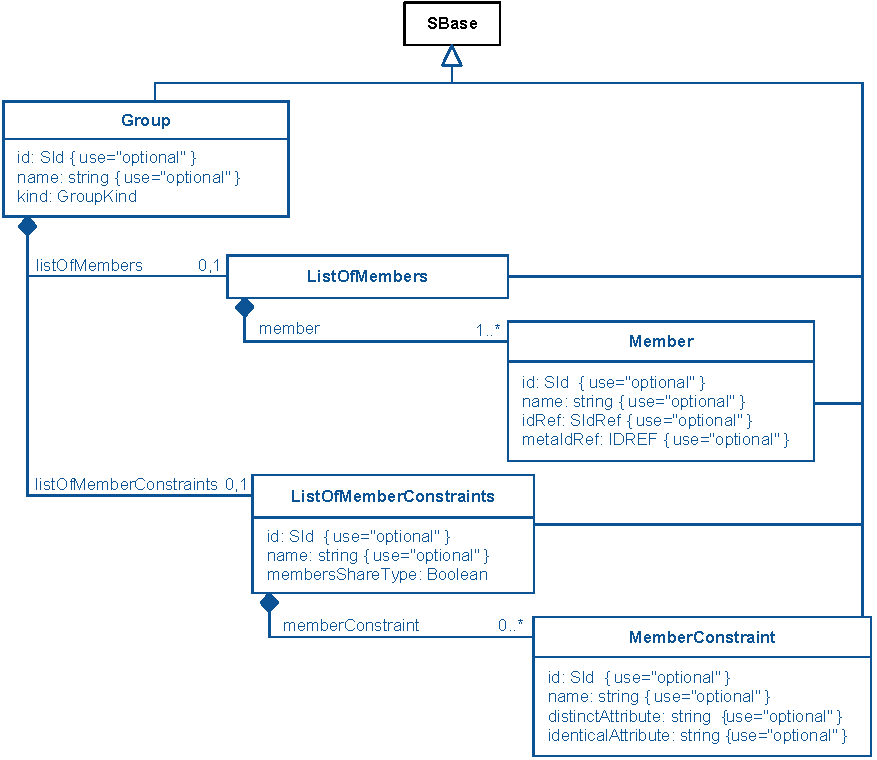
\includegraphics{figs/group-uml-v2}
  \vspace*{-1ex}
  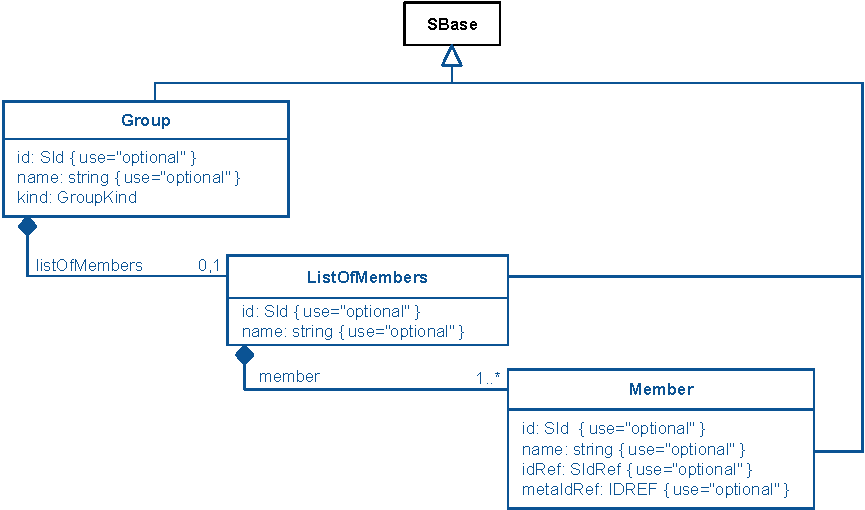
\includegraphics[scale=0.95]{figs/group-uml-v1}
%VERSION2
%\caption{The definition of the \Group, \ListOfMembers, \Member, \ListOfMemberConstraints, and \MemberConstraint classes.}
 \caption{The definition of the \Group, \ListOfMembers, and \Member classes.}
  \label{group-uml}
  \label{member-uml}
\end{figure}

\subsubsection{The \fixttspace\tokenNC{kind} attribute}
\label{kind-attribute}

\Group has one required attribute, \token{kind}, of type \primtype{GroupKind}.  This attribute is used to indicate the nature of the group defined by a \Group instance.  The \token{kind} attribute must always have one of the three possible values of \primtype{GroupKind}; these values have the following meanings:

\begin{description}[font=\normalfont\ttfamily\color{black},style=nextline]

\item[\token{classification}] The group represents a class, and its members have an \emph{is-a} relationship to the group.  For example, the group could represent a type of molecule such as ATP, and the members could be species located in different compartments, thereby establishing that the species are pools of the same molecule in different locations.

\item[\token{partonomy}] The group represents a collection of parts, and its members have a \emph{part-of} relationship to the group.  For example, the group could represent a cellular structure, and individual compartments could be made members of the group to indicate they represent subparts of that cellular structure.

\item[\token{collection}] The grouping is merely a collection for convenience, without an implied relationship between the members.  For example, the group could be used to collect together multiple disparate components of a model---species, reactions, events---involved in a particular phenotype, and apply a common annotation rather than having to copy the same annotation to each component individually.

\end{description}

\subsubsection{Group membership}
\label{group-membership}

If an SBML element is referenced by a \Group's child \Member (directly or indirectly---see below), it is considered to be a member of that \Group.  If the same element is referenced by multiple \Member objects, this is equivalent to including it just once.  It is considered best practice to avoid this, but does not make for an invalid SBML document.  Children of referenced elements are not considered to be members of the \Group: a \KineticLaw of a referenced \Reaction is not itself a \Group member.  Even the membership of SBML 'container' classes (\ListOfSpecies, \ListOfCompartments, etc.) do not imply inclusion of their children as members of the \Group.  The sole exception to this rule is the \ListOfMembers class, described below. 


\subsection{The \class{ListOfMembers} class}
\label{listofmembers-class}

The \ListOfMembers class is defined in \fig{member-uml}, and must have one or more \Member children.  Since \ListOfMembers is derived from \SBase, it inherits the \token{sboTerm} and \token{metaid} attributes, as well as the optional children \Notes and \Annotation.  Unlike most lists of objects in SBML, however, the \token{sboTerm} attribute and the \Notes and \Annotation children are taken here to apply directly to every SBML element referenced by each child \Member of this \ListOfMembers, if that referenced element has no such defin\changed{i}tion.  Thus, if a referenced element has no defined \token{sboTerm}, child \Notes, or child \Annotation, that element should be considered to now have the \token{sboTerm}, child \Notes, or child \Annotation of the \ListOfMembers.

If multiple \ListOfMembers have child \Member elements that reference the same SBML element, and more than one \ListOfMembers or \Member \changed{has a value for an} \token{sboTerm} attribute, \Notes, or \Annotation element, those \Member elements should be consistent with each other:  the \token{sboTerm} attributes should either be identical, or one should inherit from the other; \Notes should say the same or similar things; and \Annotation elements should not conflict.  Interpreters may choose to resolve any such conflicts arbitrarily.

\subsubsection{The \fixttspace\tokenNC{id} and \fixttspace\tokenNC{name} attributes}
\label{listofmembers-idname-attributes}

The optional \token{id} attribute on the \ListOfMembers object class serves to provide a way to reference the collection by its elements instead of as a collection:  the \token{id} attribute on a \Group is used for the latter, when you need to refer to the group as a group; the \token{id} of the \ListOfMembers is used when you need a short-hand way of referring to all the elements of a group at once.  The attribute takes a value of type \primtype{SId}.  Note that this identifier carries no mathematical interpretation and cannot be used in mathematical formulas in a model.

\ListOfMembers also has an optional \token{name} attribute, of type \primtype{string}.  The \token{name} attribute may be used in the same manner as other \token{name} attributes on \sbmlthreecore objects; please see Section~3.3.2 of the \sbmlthreecore specification for more information.


\subsection{The \class{Member} class}
\label{member-class}

The \Member class is defined in \fig{member-uml}.  It has four optional attributes: \token{id} and \token{name}, which identify the element, and \token{idRef} and \token{metaIdRef} which reference the identifiers of other elements.  There must be exactly \emph{one} (and only one) method used to reference another element: either \token{idRef} or \token{metaIdRef} may be defined, but not both.  (Multiple attributes are needed to account for the different types of identifiers that a given object may have.)  The referenced object (including, potentially, another \Group object) is thus made a member of the group in which the \Member object is contained.

Since \Member is derived from \SBase and, as mentioned above, \SBase provides both the ability to attach SBO terms as well as MIRIAM annotations, the semantics of a given member in a model can be made more precise by reference to external controlled vocabularies and ontologies.

The meaning and purpose of the attributes on the object class are described below.


\subsubsection{The \fixttspace\tokenNC{id} and \fixttspace\tokenNC{name} attributes}
\label{member-idname-attributes}

The optional \token{id} attribute on the \Member object class serves to provide a way to identify the member reference.  The attribute takes a value of type \primtype{SId}.  Note that the identifier of a member reference carries no mathematical interpretation and cannot be used in mathematical formulas in a model.  \Member also has an optional \token{name} attribute, of type \primtype{string}.  The \token{name} attribute may be used in the same manner as other \token{name} attributes on \sbmlthreecore objects; please see Section~3.3.2 of the \sbmlthreecore specification for more information.


\subsubsection{The \fixttspace\tokenNC{idRef} attribute}
\label{member-idref-attribute}

%VERSION2
%The attribute \token{idRef} on the \Member class has type \primtype{SIdRef}, and must be defined if the \Member has no defined \token{metaIdRef} attribute, and must not be defined otherwise.  The value must be the identifier of an object elsewhere in the \Model.  (Object identifiers are usually set by attributes named \token{id}; thus, the \token{idRef} value will usually be the \token{id} value of an object in the \Model.)  An example value of \token{idRef} might be the identifier of a species in the model, or the identifier of another group.  The namespace in which the \primtype{SId} is to be found is the SId namespace of the \Model to which the \Group belongs.  This includes elements from SBML packages which may have elements with \token{id} values that are part of the SId namespace of the \Model, such as \Deletion elements from the Hierarchical Model Composition package, \FluxBound elements from the Flux Balance Constraints package, and \Group, \Member, \ListOfMemberConstraints, and \MemberConstraint elements from this Groups package.  Conversely, elements with \token{id} values that are not part of the SId namespace of the \Model such as \Unit and \LocalParameter elements in \sbmlthreecore, or \Port elements from the Hierarchical Model Composition package, may not be referenced by this \token{idRef} attribute.
The attribute \token{idRef} on the \Member class has type \primtype{SIdRef}, and must be defined if the \Member has no defined \token{metaIdRef} attribute, and must not be defined otherwise.  The value must be the identifier of an object elsewhere in the \Model.  (Object identifiers are usually set by attributes named \token{id}; thus, the \token{idRef} value will usually be the \token{id} value of an object in the \Model.)  An example value of \token{idRef} might be the identifier of a species in the model, or the identifier of another group.  The namespace in which the \primtype{SId} is to be found is the SId namespace of the \Model to which the \Group belongs.  This may include elements from SBML packages that define elements with \token{id} values that are part of the SId namespace of the \Model.  A few examples are the \Deletion elements from the \changed{SBML Level~3} Hierarchical Model Composition package, \FluxBound elements from the Flux Balance Constraints package, and \Group and \Member elements from this Groups package.

Conversely, elements with \token{id} values that are not part of the SId namespace may not be referenced by this \token{idRef} attribute.  In \sbmlthreecore, this includes the \Unit and \LocalParameter elements.  For any SBML package, the same rule applies, such as for the \Port elements from the Hierarchical Model Composition package.


\subsubsection{The \fixttspace\tokenNC{metaIdRef} attribute}
\label{member-metaidref-attribute}

The \Member attribute \token{metaIdRef} takes a value of type \primtype{IDREF}.  The attribute must be defined if the \Member has no defined \token{idRef} attribute, and must not be defined otherwise.  This attribute is used to refer to a \token{metaid} attribute value on any other object in the \Model, for cases where the object being referenced does not have an identifier in the \Model SId namespace.  (This is the case with, for example, rules in \sbmlthreecore.)  Since meta identifiers are optional attributes of \SBase, all SBML objects have the potential to have a meta identifier value, including most elements from other SBML packages.

Note that even if used in conjunction with the \changed{SBML Level~3} Hierarchical Model Composition package, this attribute is not allowed to reference elements that reside within other \Model objects in the same SBML Document.  Referenced elements must be normal members of the parent \Model containing the \Member object, and submodel elements may be normally accessed by creating replacements.


\subsubsection{Members referencing other Groups and Members}
\label{nested-groups}

If a \Member references a \Group, it is the \Group itself that is considered to be a member of the parent \Group, not the corresponding referenced element (or elements).  This is also true for elements from other packages that point to other elements, such as \SBaseRef elements from the \changed{SBML Level~3} Hierarchical Model Composition package.  However, if a \Member references a \ListOfMembers object, it is the elements referenced in that list that are considered to be part of the parent \Group.

%VERSION2
% The implication of this is that all the rules in this specification that apply to members of a group (such as how the \token{kind} attribute functions, the application of \token{sboterm} attributes on a \ListOfMembers, and the \ListOfMemberConstraints restrictions, described below) apply to the child group itself, and not to its members.  If a parent group includes two species plus a child group which itself contains three other species, if the parent group's \ListOfMembers is given an \token{sboterm}, that term applies to the two species and the group, \emph{not} to the three child species members of the second group.  That parent group's \token{kind} would also almost certainly be \val{collection} or \val{partonomy}, and not \val{classification}, as two species and a group are very unlikely to be classified as the same thing. 
The implication of this is that all the rules in this specification that apply to members of a group (such as how the \token{kind} attribute functions, and the application of \token{sboterm} attributes on a \ListOfMembers restrictions, described below) apply to the child group when referenced by the \Group id, but to the members of the child group when referenced by the \ListOfMembers id.  In \changed{an example situation} where a parent group includes two \Species plus a \Group which itself contains three other \Species, if the parent group's \ListOfMembers is given an \token{sboterm}, that term applies to the two species \emph{and the group, not} to the three child species members of the second group.  Note that the parent group's \token{kind} would also almost certainly be \val{collection} or \val{partonomy}, and not \val{classification}, as two species and a group are very unlikely to be classified as the same thing.  In contrast, in the situation where a parent group includes two \Species plus a \ListOfMembers which contains three other \Species, the parent group's \ListOfMembers \token{sboterm} would apply to the five \Species, and could be more reasonably marked as a \val{classification}.

In a future version of this specifi\changed{c}ation, it may be possible to perform set operations on groups, but for now, this type of union is the only set operation that is possible.  For more detail, see \sec{semantics}

Finally, groups are not permitted to be circular:  no \Member may reference itself, its parent \ListOfMembers, nor its parent \Group.  If a \Member references a \Group, the same restrictions apply to that subgroup's children:  they may not reference the \Member, its parent \ListOfMembers, nor its parent \Group, and if any of those children reference a \Group, the same restrictions apply to them, etc.

\subsubsection{Members referencing other namespaces}
\label{unfindable-members}

If a \Member has a \token{idRef} or \token{metaIdRef} attribute which references an object from a namespace that is not understood by the interpreter of the SBML model, that \Member must be ignored---the referenced object will not be understood by the interpreter, and therefore has no need to become a member of the group. If an interpreter cannot tell whether a referenced object does not exist or if exists in an unparsed namespace, it may choose to produce a warning.


\subsubsection{Example}

As mentioned above, exactly one of the attributes \token{idRef} and \token{metaIdRef} must have a value in a given \Member object instance.  There are no restrictions on mixing the attributes used across multiple members of the same group, however.  The following artificial example illustrates the use of heterogeneous and nested groups.  The group \val{all\_species} references only species, but the group \val{all\_entities} references the compartment, the group of species, and the rule (the last through the use of the \token{metaIdRef} attribute):

\begin{example}
...
  <listOfSpecies>     
      <species id="S1" compartment="c" initialConcentration="1"/> 
      <species id="S2" compartment="c" initialConcentration="2"/> 
  </listOfSpecies>   
  <listOfCompartments>   
      <compartment id="C" size="1"/>
  </listOfCopartments>   
  <listOfRules>
      <rateRule variable="S2" metaid="_rule1">
          <math xmlns="http://www.w3.org/1998/Math/MathML">
              <apply>
                  <times/>
                  <ci> S1 </ci>
                  <cn> 0.5 </cn>
              </apply>
          </math>
      </rateRule>
  </listOfRules>
  <listOfGroups xmlns="http://www.sbml.org/sbml/level3/version1/groups/version1">   
      <group kind="collection">
          <listOfMembers id="all_species">
              <member idRef="S1"/> 
              <member idRef="S2"/> 
          </listOfMembers>
      </group> 
      <group id="all_entities" kind="collection">
          <listOfMembers>
              <member idRef="C"/> 
              <member idRef="all_species"/> 
              <member metaIdRef="_rule1"/> 
          </listOfMembers>
      </group> 
  </listOfGroups>   
...
\end{example}


%VERSION2
%\subsection{The \class{ListOfMemberConstraints} class}
%\label{listOfMemberConstraints-class}

%The \ListOfMemberConstraints class is defined in \fig{group-uml} as a way to impose restrictions on the referenced member elements of a \Group.  It can be used to ensure that all members of a group are of the same SBML Class or to ensure that all members of the group have the same attribute with the same value or with all different values.

%It has one required attribute, \token{membersShareType}, and two optional attributes: \token{id} and \token{name}.  It also may contain zero or more \MemberConstraint child objects, all described below.  (Allowing zero or more children lets one set the \token{membersShareType} constraint without forcing you to set other constraints.)

%\subsubsection{The \fixttspace\tokenNC{id} and \fixttspace\tokenNC{name} attributes}
%\label{listOfMemberConstraints-idname-attributes}

%The optional \token{id} attribute on the \ListOfMemberConstraints object class serves to provide a way to identify the constraints.  The attribute takes a value of type \primtype{SId}.  Note that this identifier carries no mathematical interpretation and cannot be used in mathematical formulas in a model.  \ListOfMemberConstraints also has an optional \token{name} attribute, of type \primtype{string}.  The \token{name} attribute may be used in the same manner as other \token{name} attributes on \sbmlthreecore objects; please see Section~3.3.2 of the \sbmlthreecore specification for more information.


%\subsubsection{The \fixttspace\tokenNC{membersShareType} attribute}
%\label{memberssharetype-attribute}

%The required attribute \token{membersShareType} on the \ListOfMemberConstraints class has type \primtype{boolean}.  If set to \val{true}, all referenced members of the \Group must be the same exact SBML class.  This means that sharing a base class (such as \SBase or \Rule) is insufficient: an \AlgebraicRule and a \RateRule are different classes from one another.

%If set to \val{false}, the referenced members of the \Group may be of any SBML class; no restrictions are implied.

%This restriction can only be violated if there are two or more members of the group.


%\subsection{The \class{MemberConstraint} class}
%\label{memberConstraint-class}

%The \MemberConstraint class is defined in \fig{group-uml} as a way to impose restrictions on common attributes of the referenced members of the \Group.  It has two optional attributes to identify the attribute constraint itself (\token{id} and \token{name}), and two other attributes (\token{identicalAttribute} and \token{distinctAttribute}) of which exactly \emph{one} (and only one) must be defined.

%\subsubsection{The \fixttspace\tokenNC{id} and \fixttspace\tokenNC{name} attributes}
%\label{memberConstraint-idname-attributes}

%The optional \token{id} attribute on the \MemberConstraint object class serves to provide a way to identify the \MemberConstraint.  The attribute takes a value of type \primtype{SId}.  Note that this identifier carries no mathematical interpretation and cannot be used in mathematical formulas in a model.  \MemberConstraint also has an optional \token{name} attribute, of type \primtype{string}.  The \token{name} attribute may be used in the same manner as other \token{name} attributes on \sbmlthreecore objects; please see Section~3.3.2 of the \sbmlthreecore specification for more information.


%\subsubsection{The \fixttspace\tokenNC{distinctAttribute} attribute}
%\label{distinctattribute-attribute}

%The attribute \token{distinctAttribute} on the \MemberConstraint class has type \primtype{string}.  This attribute must be defined if the \MemberConstraint has no defined \token{identicalAttribute}, and must not be defined otherwise.  The value of the string must be the name of an attribute shared by all referenced members of the \Group.  Furthermore, the \emph{values} of those attribute must be different across all referenced elements.  The rule from SBML Level~2 that no two \SpeciesType elements may share a compartment could be replicated here by setting this attribute to \val{compartment}.

%If the referenced attribute exists in a particular namespace, the namespace should be included as part of the string, with a colon separting it from the text of the attribute name itself (i.e. \val{groups:idRef}).

%This restriction can only be violated if there are two or more members of the group.


%\subsubsection{The \fixttspace\tokenNC{identicalAttribute} attribute}
%\label{identicalattribute-attribute}

%The attribute \token{identicalAttribute} on the \MemberConstraint class has type \primtype{string}.  This attribute must be defined if the \MemberConstraint has no defined \token{distinctAttribute}, and must not be defined otherwise.  The value of the string must be the name of an attribute shared by all referenced members of the \Group.  Furthermore, the \emph{values} of those attributes must be the same for all referenced elements.  If the referenced members are all \Species, for example, this attribute might be set to be \val{boundaryCondition}, ensuring that all the referenced elements have the same value (\val{true} or \val{false}).  To ensure that all of these species had the same units, another \MemberConstraint could be set with an \token{identicalAttribute} of \val{substanceUnits}.

%If the referenced attribute exists in a particular namespace, the namespace should be included as part of the string, with a colon separting it from the text of the attribute name itself (i.e. \val{groups:idRef}).

%This restriction can only be violated if there are two or more members of the group.


%\subsubsection{Example}

%A partial example of a working \ListOfMemberConstraints element is shown below.  In it, the two referenced members (\val{ATPc} and \val{ATPm}) are declared to be the same type using the \token{membersShareType} attribute, that they must have different compartments with a \token{distinctAttribute} attribute, and that they must both have the same units with a \token{identicalAttribute} attribute. 

%\clearpage

%\begin{example}
%    <group id="ATP" kind="classification"> 
%        <listOfMembers sboTerm="SBO:0000248">
%            <member idRef="ATPc" />
%            <member idRef="ATPm" />
%        </listOfMembers>
%        <listOfMemberConstraints membersShareType="true">
%            <memberConstraint distinctAttribute="compartment" />
%            <memberConstraint identicalAttribute="substanceUnits" />
%        </listOfMemberConstraints>
%    </group> 
%\end{example}

%A complete SBML document including the above snippet is included in \sec{examples-speciestype}.

\subsection{The extended \class{Model} class}
\label{model-class}
\label{extended-model-class}
\label{listofgroups-class}

The Groups package extends \sbmlthreecore's \Model class to add one list, \ListOfGroups, for holding group definitions.  \fig{extended-model-uml} provides the UML diagram for the extension.

\begin{figure}[hbt]
  \begin{overpic}{figs/group-model-uml}
    \put(85.25,12.75){\emph{\sec*{group-class}}}
  \end{overpic}
  \caption{The extensions of the \Model class.  \Group is defined in \sec{group-class}. In other respects, \Model remains defined as in the \sbmlthreecore specification.}
  \label{extended-model-uml}
\end{figure}


\subsubsection{The list of groups}

\fig{extended-model-uml} shows that the extension of \Model by the Groups package involves adding an optional \token{listOfGroups} subcomponent for holding a \ListOfGroups container object.  If present, the \ListOfGroups instance must contain at least one \Group object (\sec{group-class}).  In common with other \textsf{\textbf{ListOf\rule{0.15in}{0.5pt}}} classes in SBML, \ListOfGroups is derived from \SBase.  It inherits \SBase's attributes \token{metaid} and \token{sboTerm}, as well as the subcomponents for \Annotation and \Notes, but does not add any new attributes of its own.


\section{The semantics of ``groups''}
\label{semantics}

A group \emph{G} is defined by declaring an instance of a \Group class object within the \ListOfGroups element of a \Model object. The group can be given an optional identifier (i.e., a value for its \token{id} attribute), but even if the group does not have an identifier, the act of declaring a group has the effect of creating it.

An entity \emph{X} in the model is declared to be part of group \emph{G} by listing the identifier of \emph{X} in a \Member object within the \ListOfGroups instance of \emph{G}, \changed{or by listing the identifier of a \ListOfMembers object of a group to which \emph{X} belongs as a \Member object of \emph{G} (thus 'nesting' the members of the subgroup)}. The following is an example to illustrate \changed{an un-nested} structure:

\begin{example}
<model id="model_1"> 
  <listOfSpecies> 
    <species id="s1" .../> 
    <species id="s2" .../> 
    <species id="s3" .../> 
    <species id="s4" .../> 
  </listOfSpecies> 
  ... 
  <listOfReactions> 
    <reaction id="r1" ...> ... </reaction> 
    <reaction id="r2" ...> ... </reaction> 
  <listOfReactions> 
  ... 
  <listOfGroups xmlns="http://www.sbml.org/sbml/level3/version1/groups/version1"> 
    <group id="some_species_group" kind="collection"> 
      <listOfMembers> 
        <member idRef="s1"/> 
        <member idRef="s3"/> 
      </listOfMembers> 
    </group> 
    <group id="some_reaction_group" kind="collection"> 
      <listOfMembers> 
        <member idRef="r1"/> 
        <member idRef="r2"/> 
      </listOfMembers> 
    </group> 
  </listOfGroups> 
</model>
\end{example}

For any given group, the meaning of group membership is determined by the value of the attribute \token{kind} on the \Group object instance.  Examples of possible meanings are given in \sec{kind-attribute}.

The meaning of a group can be further refined by using annotations (either SBO terms or the \Annotation element) on the group, or the list of members. This possibility raises the question of how the annotations should be interpreted across the group members.  The following are the possibilities defined by the Groups package (summarizing \sec{group-class}, \sec{listofmembers-class}, and \sec{member-class}):

\begin{itemize}

\item If the annotation or SBO term is on a \Group object, it is an annotation about the group itself, not the individual members.

\item If the annotation or SBO term is on a \Member object, it is an annotation about the \Member itself, and not about its referenced element.

\item If the annotation or SBO term is on \ListOfMembers, it is a short-hand that means the annotation applies to each individual referenced member, as if the annotation were put on the referenced SBML elements directly.

\end{itemize}

Similar rules apply to nested groups:

\begin{itemize}

\item If a \Group object is referenced by a \Member, it is the group itself that is included in that \Member's parent \Group, not its individual members.

\item If a \Member object is referenced by another \Member, it is that member that is included in the parent \Group, and not the referenced SBML element to which the \Member points.

\item If a \ListOfMembers object is ref\changed{er}enced by a \Member, all of the referenced SBML elements from that \ListOfMembers are included in the parent \Group.  It is equivalent to including all of the referenced elements directly.

\end{itemize}

\changed{The following example uses the above rules to nest the members of group1 inside group2, using the \val{group1\_list} \ListOfMembers id:}


\begin{example}
<model id="model_2"> 
  ... 
  <listOfGroups xmlns="http://www.sbml.org/sbml/level3/version1/groups/version1"> 
    <group id="group1"> 
      <listOfMembers id="group1_list"> 
        <member idRef="..."/> 
        <member idRef="..."/> 
      </listOfMembers> 
    </group> 
    <group id="group2"> 
      <listOfMembers> 
        <member idRef="group1_list"/> 
        <member idRef="..."/> 
        <member idRef="..."/> 
      </listOfMembers> 
    </group> 
  </listOfGroups> 
</model> 
\end{example}

The intended meaning of nested groups can be made more precise by annotating the group and list of members with \changed{appropriate annotations} using controlled vocabulary terms that describe the meaning.


\subsection{Semantic restrictions}
\label{semantic-restrictions}

The current definition of the Groups package is such that the use of Groups constructs has no impact on the mathematics of a model.  As a consequence of this, this package is not required for proper interpretation of a model. The document must use the \token{required}=\val{false} flag on the declaration of the package on the \token{<sbml>} element in a file.

%VERSION2
%Because restrictions can be imposed on the group through the use of the \ListOfMemberConstraints element, the Groups package can fully recapture SBML Level~2's \SpeciesType construct: to do so, the group's \token{kind} attribute should be set to \val{classification}, a \ListOfMemberConstraints should be added with its \token{membersShareType} attribute set to \val{true}, and it should be given a child \MemberConstraint with its \token{distinctAttribute} attribute set to \val{compartment}.  A fully worked example (which also imposes additional restrictions) is given in \sec{examples-speciestype}.
